% -*- root: projekt.tex -*-

%\chapter{Obsah CD}
%\chapter{Manual}
%\chapter{Konfigrační soubor}
%\chapter{RelaxNG Schéma konfiguračního soboru}
%\chapter{Plakat}

\chapter{Uživatelská příručka}
\label{apxManual}

\section{Překlad programu}

Program je rozdělen do několika modulů. Jejich překlad a sestavení výsledného programu je definován v~Makefile a spouští se příkazem \texttt{make}. Je potřeba překladač GCC ve verzi alespoň 4.8, lépe ve verzi 4.9, která má dokonalejší podporu SIMD instrukcí, zejména umí využít všechny dostupné registry. Kvůli některým použitým funkcím (např. pro získání spotřebovaného procesorového času) musí operační systém implementovat standard POSIX. Program byl testován na systémech Ubuntu 12.04 a na superpočítači Anselm, který používá systém bullx Linux odvozený od Red Hat Enterprise Linux.

Pokud překlad končí chybou a na výstupu jsou takovéto zprávy:

\begin{lstlisting}[language=]
/tmp/ccQ9hvQS.s: Assembler messages:
/tmp/ccQ9hvQS.s:33: Error: suffix or operands invalid for `vpcmpeqd'
/tmp/ccQ9hvQS.s:85: Error: suffix or operands invalid for `vpcmpeqd'
/tmp/ccQ9hvQS.s:92: Error: suffix or operands invalid for `vpcmpeqd'
\end{lstlisting}

\noindent{}je třeba z Makefile odstranit z proměnné \texttt{CFLAGS} část \texttt{-DAVX2}, čímž se vypne kompilace kódu akcelerovaného pomocí instrukcí AVX2. Chyby jsou s největší pravděpodobností způsobeny tím, že použitý překladač je novější verze a generuje kód, kterému použitý assembler nerozumí\footnote{viz http://code.compeng.uni-frankfurt.de/issues/718}. Tento problém se vyskytl na Anselmu, jehož procesory instrukce AVX2 nepodporují.

Jednotlivé moduly programu se překládají samostatně do složky \texttt{build}. Při změnách ve zdrojovém kódu tak není nutné opakovaně překládat moduly, do kterých se nezasahovalo. Výstupem překladu je několik spustitelných souborů:

\begin{itemize}
    \item \texttt{coco}\footnote{Název \texttt{coco} je zkratka pro COlearning in COevolution.} -- hlavní program, samotný evoluční návrh obrazových filtrů,
    \item \texttt{coco\_apply} -- aplikace filtru uloženého v~souboru \texttt{*.chr} na libovolný obrázek,
    \item \texttt{coco\_predvis} -- vizualizace použitých prediktorů fitness,
    \item \texttt{coco\_predhist} -- tvorba histogramu pixelů používaných v~prediktorech fitness.
\end{itemize}

\section{Formáty souborů}

\subsubsection*{Obrázky}

Načítání trénovacích obrázků je řešeno pomocí knihovny \texttt{stb\_image.h}\footnote{\url{https://github.com/nothings/stb}}. Jsou tedy podporovány formáty implementované v~této knihovně, s~většími či menšími omezeními: JPEG, PNG, TGA, BMP, PSD, GIF, HRD, PIC. Všechny obrázky musí být uloženy ve stupních šedi, 8 bitů na pixel. Testovány byly pouze obrázky ve formátech BMP a PNG. Výstupní obrázky (např. výstup nejlepšího filtru) jsou ukládány vždy ve formátu PNG.

\subsubsection*{Obrazové filtry}

Chromozomy obrazových filtrů jsou ukládány do textového formátu, který je totožný s~formátem, který používá program CGP Viewer, který vypadá takto:

\begin{lstlisting}
{2, 2, 4, 1, 2, 1, 16}                                  %*\Comment{Konfigurace CGP}*
([3] 0, 1, 2)([4] 2, 1, 2)([5] 0, 2, 13)([6] 3, 4, 6)   %*\Comment{Vstupy a funkce bloků}*
(5, 4)                                                  %*\Comment{Primární výstupy}*
\end{lstlisting}

Na začátku je ve složených závorkách uvedena konfigurace mřížky a funkčních bloků: počet primárních vstupů, primárních výstupů, šířka a výška mřížky, počet vstupů a výstupů funkčních bloků a počet možných funkcí, které může blok vykonávat. Dále jsou pro každý blok v~kulatých závorkách uvedeny jeho číslo (v~hranatých závorkách) a jeho geny: čísla bloků, na které jsou připojené jeho vstupy a číslo funkce, kterou vykonává. Na závěr jsou v~kulatých závorkách uvedeny čísla bloků, kam jsou připojeny primární výstupy programu.

Kromě tohoto formátu jsou filtry ukládány také jako kód v~jazyce C a v~textovém formátu srozumitelném pro uživatele, který pro stejný program vypadá takto:

{
    \centering
    \vskip\baselineskip
    \begin{BVerbatim}[fontsize=\footnotesize]
         .------------------------------------------------------------------------.
         |      .----.            .----.            .----.            .----.      |
    [ 0]>| [ 0]>|    |>[ 2]  [ 2]>|    |>[ 3]  [ 0]>|    |>[ 4]  [ 3]>|    |>[ 5] |>[5]
    [ 1]>| [ 1]>| f2 |       [ 1]>| f2 |       [ 2]>| f13|       [ 4]>| f6 |      |>[4]
         |      '----'            '----'            '----'            '----'      |
         '------------------------------------------------------------------------'
    \end{BVerbatim}
}

\section{Spuštění evoluce obrazových filtrů}

Povinné parametry jsou pouze dva, a sice:

\begin{itemize}
    \item \texttt{-{}-noisy SOUBOR} nebo \texttt{-n SOUBOR}
    \item \texttt{-{}-original SOUBOR} nebo \texttt{-i SOUBOR}
\end{itemize}

Jména souborů se zdrojovým (poškozeným) a cílovým (nepoškozeným) obrázkem. V~případě detekce hran se u~parametru \texttt{-{}-noisy} uvede zdrojový obrázek a u~\texttt{-{}-original} obrázek s~vyznačenými hranami.

Ostatní parametry jsou volitelné, pokud nejsou uvedeny, použije se výchozí hodnota.

\subsection{Parametry evoluce}

\newcommand\cmdarglist[1]{
    \begin{description}#1\end{description}
}

\newcommand\cmdarg[2]{
    \item[\texttt{#1}] \hfill \\
    #2
}

\newcommand\cmdargdef[3]{
    \item[\texttt{#1}] (výchozí: #2) \hfill \\
    #3
}

\cmdarglist{
    \cmdargdef{-{}-algorithm ALG, -a ALG}{\texttt{coev}}{
        Algoritmus evoluce.
        \begin{itemize}
            \item \texttt{cgp} -- standardní CGP,
            \item \texttt{coev} -- koevoluce s~pevnými prediktory fitness,
            \item \texttt{colearn} -- koevoluce se souběžným učením.
        \end{itemize}
    }

    \cmdargdef{-{}-random-seed N, -r N}{dle \texttt{gettimeofday()}}{
        Inicializační hodnota generátoru pseudonáhodných čísel.
    }

    \cmdarg{-{}-target-psnr N, -t N}{
        Evoluce se ukončí po dosažení zvolené hodnoty PSNR.
    }

    \cmdarg{-{}-target-fitness N, -f N}{
        Evoluce se ukončí po dosažení zvolené fitness. Jde o~hodnotu zlomku ve výpočtu PSNR, jak je uvedeno v části~\ref{secImplFitness}.
    }
}

\subsection{Parametry sběru dat}

\cmdarglist{
    \cmdarg{-{}-log-dir DIR, -l DIR}{
        Složka, do které se uloží záznamy o~běhu. Pokud neexistuje, bude vytvořena. Její obsah popisuje sekce \ref{apxManualLogDir}.
    }

    \cmdarg{-{}-log-interval N, -k N}{
        Kromě záznamů při změně fitness filtru, zapíše do logu také každou N-tou generaci.
    }

    \cmdarg{-{}-log-pred-file FILE}{
        Do souboru \texttt{FILE} zapíše obsah všech prediktorů použitých při ohodnocování fitness. Soubor lze dále zpracovat nástroji \texttt{coco\_predhist} a \texttt{coco\_predvis}.
    }
}

\subsection{Parametry populace obrazových filtrů}

\cmdarglist{
    \cmdargdef{-{}-cgp-mutate N, -m N}{5}{
        Maximální počet pozměněných genů filtru při mutaci.
    }

    \cmdargdef{-{}-cgp-population-size N, -p N}{8}{
        Počet jedinců v~populaci filtrů.
    }

    \cmdargdef{-{}-cgp-archive-size N, -s N}{8}{
        Velikost archivu filtrů pro ohodnocování prediktorů.
    }
}

\subsection{Parametry populace prediktorů fitness}

\cmdarglist{
    \cmdargdef{-{}-pred-size N, -S N}{0,25}{
        Velikost genotypu prediktorů v~procentech (jako desetinné číslo). V~případě souběžného učení je vhodné uvést hodnotu 1.
    }

    \cmdargdef{-{}-pred-mutate N, -M N}{5}{
        Maximální procento pozměněných genů prediktoru při mutaci.
    }

    \cmdargdef{-{}-pred-population-size N, -P N}{32}{
        Počet jedinců v~populaci prediktorů.
    }

    \cmdargdef{-{}-pred-type TYPE, -T TYPE}{\texttt{permuted} nebo \texttt{repeated} dle \texttt{-{}-algorithm}}{
        Typ prediktoru:
        \begin{itemize}
            \item \texttt{permuted} -- genotyp bez duplicitních genů, výchozí pro koevoluci s~fixními prediktory (\texttt{-a coev}), nelze použít při souběžném učení,
            \item \texttt{repeated} -- s~duplicitními geny, výchozí pro souběžné učení (\texttt{-a colearn}),
            \item \texttt{repeated-circular} -- s~duplicitními geny, offset tvorby fenotypu se určí jako nejlepší z~5 náhodných možností.
        \end{itemize}
    }
}

\subsection{Parametry souběžného učení}



\chapter{Výsledky experimentů}
\label{apxResults}

\section{Úprava velikosti prediktoru podle celkového počtu případů fitness}
\label{apxExpAbs}

Následující grafy se týkají varianty souběžného učení, kdy je přírůstek nebo úbytek velikosti prediktoru relativní k~celkovému počtu případů fitness. Používají se pravidla uvedená v~tabulce \ref{tabBaldwinRulesAbs}. Experimentovalo se s~různými hodnotami koeficientů $c_0$, $c_{-1}$, $c_{+1}$ a $c_{+2}$, konkrétně od $-0.10$ po $+0.10$ s~krokem po $0.01$. Trénovací obrázek byl poškozen šumem typu sůl a pepř o~intenzitě 15\,\%.

{
\captionsetup{aboveskip=0pt}

\begin{figure}[h]
    \centering
    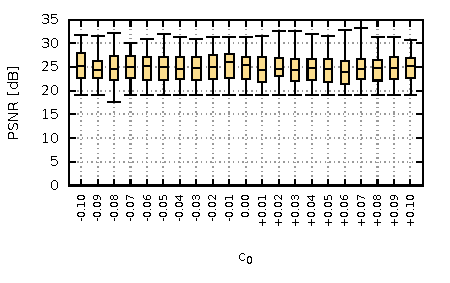
\includegraphics[width=0.475\textwidth]{fig/plot/tuningabs-zeroinc-30kg-psnr.pdf}
    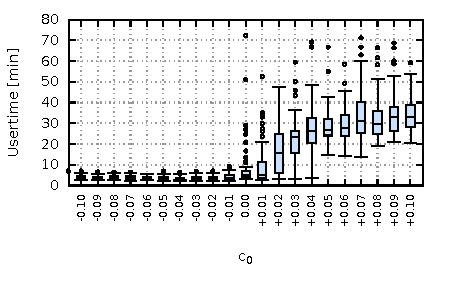
\includegraphics[width=0.475\textwidth]{fig/plot/tuningabs-zeroinc-30kg-utime.pdf}
    \caption{Vliv parametru $c_{0}$ (pravidlo $\left|v\right| \leq v_\mathit{zero}: \mathit{UsedGenes} \leftarrow \mathit{UsedGenes} + \left(N \cdot c_0\right)$}
\end{figure}

\begin{figure}[h]
    \centering
    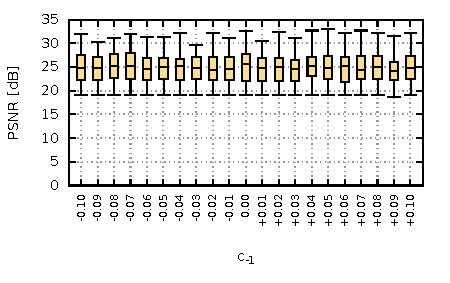
\includegraphics[width=0.475\textwidth]{fig/plot/tuningabs-decrinc-30kg-psnr.pdf}
    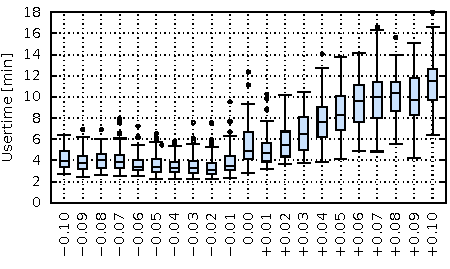
\includegraphics[width=0.475\textwidth]{fig/plot/tuningabs-decrinc-30kg-utime.pdf}
    \caption{Vliv parametru $c_{-1}$ (pravidlo $v < 0: \mathit{UsedGenes} \leftarrow \mathit{UsedGenes} + \left(N \cdot c_{-1}\right)$}
\end{figure}

\begin{figure}[h]
    \centering
    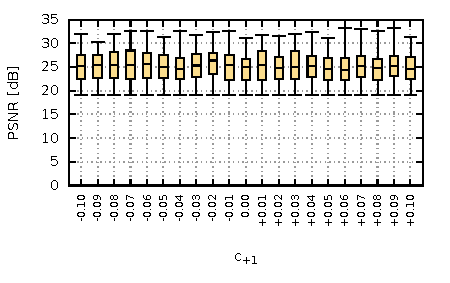
\includegraphics[width=0.475\textwidth]{fig/plot/tuningabs-slowinc-30kg-psnr.pdf}
    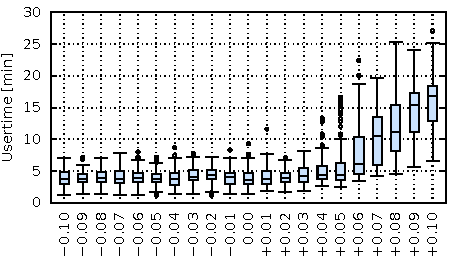
\includegraphics[width=0.475\textwidth]{fig/plot/tuningabs-slowinc-30kg-utime.pdf}
    \caption{Vliv parametru $c_{+1}$ (pravidlo $0 < v~\leq v_\mathit{slow}: \mathit{UsedGenes} \leftarrow \mathit{UsedGenes} + \left(N \cdot c_{+1}\right)$}
\end{figure}

\begin{figure}[h]
    \centering
    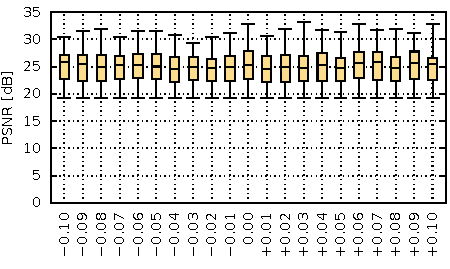
\includegraphics[width=0.475\textwidth]{fig/plot/tuningabs-fastinc-30kg-psnr.pdf}
    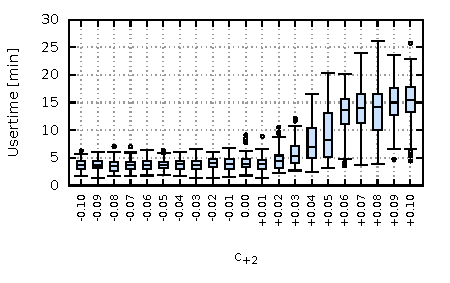
\includegraphics[width=0.475\textwidth]{fig/plot/tuningabs-fastinc-30kg-utime.pdf}
    \caption{Vliv parametru $c_{+2}$ (pravidlo $v > v_\mathit{slow}: \mathit{UsedGenes} \leftarrow \mathit{UsedGenes} + \left(N \cdot c_{+2}\right)$}
\end{figure}

}
